\documentclass[10pt, spanish, twocolumn]{article}

% --- Paquetes de Diseño Editorial NYT ---
\usepackage[utf8]{inputenc}
\usepackage[T1]{fontenc}
\usepackage{babel}
\usepackage{amsmath, amssymb, amsfonts}
\usepackage{libertinus}
\usepackage[default]{montserrat}
\usepackage{microtype}
\usepackage[margin=1.5cm, top=2.5cm, bottom=2cm, columnsep=0.8cm]{geometry}

% --- Gráficos y Diagramas ---
\usepackage{tikz}
\usepackage{pgfplots}
\pgfplotsset{compat=1.18}
\usetikzlibrary{patterns, arrows.meta, positioning, shapes.geometric, circuits.ee.IEC}

% --- Paleta de Colores "The New York Times" ---
\usepackage{xcolor}
\definecolor{nytblack}{RGB}{18, 18, 18}
\definecolor{nytgray}{RGB}{120, 120, 120}
\definecolor{accentblue}{RGB}{50, 104, 145}
\definecolor{accentred}{RGB}{204, 0, 0}
\definecolor{accentgreen}{RGB}{0, 128, 96}
\definecolor{accentorange}{RGB}{230, 126, 34}

% --- Ingeniería de Títulos Estilo "Magazine" ---
\usepackage[explicit]{titlesec}
\titleformat{\section}
  {\normalfont\bfseries\sffamily\Large\color{nytblack}}
  {}{0pt}{\MakeUppercase{#1}}[{\color{nytblack}\titlerule[1.5pt]}]
\titleformat{\subsection}
  {\normalfont\bfseries\sffamily\normalsize\color{accentblue}}
  {}{0pt}{#1}
\titleformat{\subsubsection}
  {\normalfont\bfseries\sffamily\small\color{accentgreen}}
  {}{0pt}{#1}

% --- Letra Capital Gigante ---
\usepackage{lettrine}
\renewcommand{\LettrineFontSpec}{\itshape\color{nytblack}}

% --- Cajas de Contenido ---
\usepackage[most]{tcolorbox}
\newtcolorbox{briefbox}[1]{
    enhanced,
    colback=white,
    colframe=nytblack!20,
    arc=0mm,
    boxrule=0.5pt,
    leftrule=3pt,
    fonttitle=\sffamily\bfseries\small,
    coltitle=nytblack,
    title=#1,
    attach title to upper,
    after title={ \textbar \ },
    drop fuzzy shadow
}

\newtcolorbox{theorembox}[1]{
    enhanced,
    colback=accentblue!5,
    colframe=accentblue,
    arc=0mm,
    boxrule=1pt,
    fonttitle=\sffamily\bfseries\small,
    coltitle=white,
    title=#1,
    attach title to upper={},
    drop fuzzy shadow
}

\newtcolorbox{examplebox}[1]{
    enhanced,
    colback=accentgreen!5,
    colframe=accentgreen!80,
    arc=0mm,
    boxrule=0.8pt,
    fonttitle=\sffamily\bfseries\small,
    coltitle=nytblack,
    title=#1,
    attach title to upper,
    after title={ \\ },
}

\newtcolorbox{warningbox}[1]{
    enhanced,
    colback=accentred!5,
    colframe=accentred,
    arc=0mm,
    boxrule=1.2pt,
    leftrule=4pt,
    fonttitle=\sffamily\bfseries\small,
    coltitle=accentred,
    title=#1,
    attach title to upper,
    after title={ \\ },
}

% --- Header Estilo Periódico ---
\usepackage{fancyhdr}
\pagestyle{fancy}
\fancyhf{}
\fancyhead[C]{\small\sffamily\textbf{THE SCIENCE TIMES} \quad \textbar \quad \textbf{MATHEMATIK FÜR INGENIEURE}}
\fancyfoot[C]{\thepage}
\renewcommand{\headrulewidth}{0.8pt}

\begin{document}

% --- Portada de Sección Mega Increíble ---
\twocolumn[
  \begin{center}
    \vspace*{-1cm}
    {\fontsize{48}{53}\selectfont\textbf{Fundamentos}} \\
    {\fontsize{48}{53}\selectfont\textbf{Matemáticos}} \\
    \vspace{0.3cm}
    {\LARGE \textit{El lenguaje riguroso que construye la ingeniería moderna.}} \\
    \vspace{0.4cm}
    {\large \sffamily Por Emanuel Quintana Silva | UPTC} \\
    {\small \sffamily ORCID: 0009-0006-8419-2805 | emanuel.quintana@uptc.edu.co} \\
    \vspace{0.7cm}
    \begin{minipage}{0.9\textwidth}
        \centering
        \hrule height 1.2pt \vspace{2pt} \hrule height 0.5pt
        \vspace{0.2cm}
        \small\sffamily \textbf{INVESTIGACIÓN ESPECIAL} \quad $\bullet$ \quad PAPULA BAND 1 \quad $\bullet$ \quad ENERO 2026
        \vspace{0.2cm}
        \hrule height 0.5pt \vspace{2pt} \hrule height 1.2pt
    \end{minipage}
    \vspace{1cm}
  \end{center}
]

% --- SECCIÓN 1: TEORÍA DE CONJUNTOS ---
\lettrine[lines=3, findent=2pt, nindent=0pt]{L}{a} transición del pensamiento escolar a la estructura de las disciplinas científicas superiores requiere más que fórmulas; exige un marco lógico riguroso que funcione como fundamento inquebrantable. Basado en la obra monumental de Lothar Papula, \textit{Mathematik für Ingenieure und Naturwissenschaftler}, la teoría de conjuntos se presenta no como un tema periférico, sino como el \textbf{átomo conceptual} sobre el cual se construye todo el edificio matemático moderno.

\section{Ontología de la Unidad}

Un conjunto es la agrupación de objetos bien diferenciados en una unidad conceptual. Esta definición, aparentemente elemental, constituye la piedra angular del análisis matemático y establece el fundamento para todas las estructuras algebraicas superiores utilizadas en ingeniería y ciencias naturales.

\begin{briefbox}{PRINCIPIO DE PERTENENCIA ABSOLUTA}
    Para que un sistema califique como conjunto válido, la relación de pertenencia debe ser absoluta y verificable sin ambigüedad. No existen zonas grises: un elemento pertenece ($\in$) o es completamente ajeno ($\notin$) al conjunto. Esta dicotomía lógica es fundamental.
\end{briefbox}

\subsection{Características Estructurales Esenciales}

Los elementos constituyentes de un conjunto deben satisfacer dos condiciones ineludibles: ser \textbf{distintos entre sí} (sin duplicados) y estar \textbf{bien diferenciados} (sin ambigüedad en su identidad). Una propiedad crucial es que el \textbf{orden de enumeración carece de relevancia lógica}, estableciendo así una estructura simétrica fundamental que distingue a los conjuntos de otras estructuras como las tuplas ordenadas.

\section{Dualidad Representacional}

En el diseño científico riguroso, la claridad de representación es un valor supremo. Los conjuntos se manifiestan en dos formas complementarias, cada una optimizada para contextos específicos.

\subsection{Método Descriptivo (Intensional)}

Define la esencia del conjunto mediante una propiedad característica. Este es el método obligatorio para sistemas infinitos donde la enumeración completa resulta imposible o impráctica.

\[ M = \{x \mid x \text{ satisface la propiedad } E \} \]

Este método aprovecha el poder del lenguaje lógico-matemático para capturar la esencia abstracta del conjunto. Por ejemplo, el conjunto de números naturales se define como $\mathbb{N} = \{x \mid x \in \mathbb{Z} \text{ y } x \geq 0\}$.

\subsection{Método Enumerativo (Extensional)}

Representa el listado directo y explícito de todos los elementos. Proporciona evidencia tangible y concreta para colecciones finitas.

\[ M_3 = \{ -3, -2, -1, 0, 1, 2, 3 \} \]

La enumeración explícita elimina toda ambigüedad interpretativa y permite verificación inmediata de pertenencia mediante inspección directa.

\section{Operaciones Fundamentales entre Conjuntos}

Las operaciones entre conjuntos (Mengenoperationen) constituyen el álgebra fundamental que permite construir estructuras matemáticas arbitrariamente complejas a partir de unidades elementales simples.

\subsection{Intersección: La Lógica Conjuntiva}

La \textbf{intersección} de dos conjuntos $A$ y $B$, simbolizada como $A \cap B$, representa el conjunto de elementos que pertenecen simultáneamente a ambos conjuntos.

\begin{theorembox}{DEFINICIÓN FORMAL DE INTERSECCIÓN}
\[ A \cap B = \{x \mid x \in A \text{ y } x \in B\} \]
\end{theorembox}

La intersección captura la noción lógica del operador "Y" (conjunción), siendo fundamental en la resolución de sistemas de inecuaciones.

\begin{examplebox}{APLICACIÓN EN SISTEMAS DE INECUACIONES}
Considere el sistema:
\begin{align*}
2x - 4 &> 0 \quad \Rightarrow \quad x > 2 \\
x &< 3
\end{align*}
La solución es la intersección de ambos conjuntos solución:
$$L = \{x \mid 2 < x < 3\} = (2,3)$$
Este intervalo abierto representa todos los valores que satisfacen simultáneamente ambas condiciones.
\end{examplebox}

\begin{center}
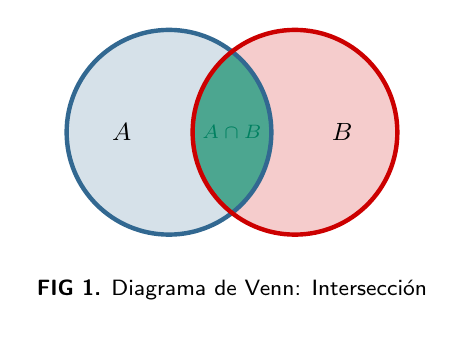
\begin{tikzpicture}[scale=1]
    \fill[accentblue!20] (0,0) circle (1.3cm);
    \fill[accentred!20] (1.6,0) circle (1.3cm);
    \begin{scope}
        \clip (0,0) circle (1.3cm);
        \fill[accentgreen!70] (1.6,0) circle (1.3cm);
    \end{scope}
    \draw[accentblue, ultra thick] (0,0) circle (1.3cm);
    \draw[accentred, ultra thick] (1.6,0) circle (1.3cm);
    \node at (-0.6, 0) {\small\sffamily\textbf{$A$}};
    \node at (2.2, 0) {\small\sffamily\textbf{$B$}};
    \node[accentgreen] at (0.8, 0) {\scriptsize\sffamily $A \cap B$};
    \node at (0.8, -2) {\footnotesize\sffamily\textbf{FIG 1.} Diagrama de Venn: Intersección};
\end{tikzpicture}
\end{center}

\subsection{Unión: La Lógica Disyuntiva Inclusiva}

La \textbf{unión} de conjuntos $A$ y $B$, denotada $A \cup B$, agrupa todos los elementos que pertenecen al menos a uno de los conjuntos.

\begin{theorembox}{DEFINICIÓN FORMAL DE UNIÓN}
\[ A \cup B = \{x \mid x \in A \text{ o } x \in B\} \]
\end{theorembox}

El operador "o" es \textbf{inclusivo}: los elementos comunes a ambos conjuntos forman parte integral de la unión, a diferencia de la disyunción exclusiva.

\begin{examplebox}{EJEMPLO CON CONJUNTOS FINITOS}
Sean $A = \{1, 2, 3, 4\}$ y $B = \{1, 5, 6, 7\}$. La unión produce:
\[ A \cup B = \{1, 2, 3, 4, 5, 6, 7\} \]
Observe que el elemento común (1) aparece una sola vez en la unión.
\end{examplebox}

\begin{examplebox}{UNIÓN DE INTERVALOS CONTINUOS}
Para $M_1 = \{x \mid 0 \le x \le 1\}$ y $M_2 = \{x \mid 1 \le x \le 5\}$:
\[ M_1 \cup M_2 = \{x \mid 0 \le x \le 5\} = [0,5] \]
Los intervalos se fusionan en uno continuo al compartir el punto frontera $x=1$.
\end{examplebox}

\begin{center}
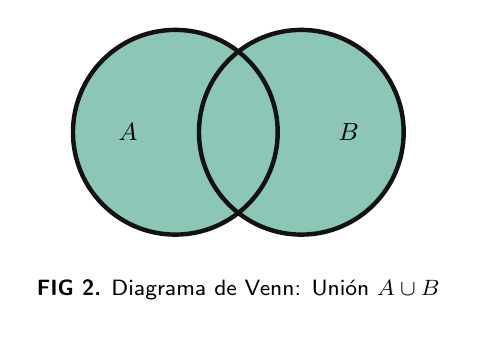
\begin{tikzpicture}[scale=1]
    \fill[accentgreen!45] (0,0) circle (1.3cm);
    \fill[accentgreen!45] (1.6,0) circle (1.3cm);
    \draw[nytblack, ultra thick] (0,0) circle (1.3cm);
    \draw[nytblack, ultra thick] (1.6,0) circle (1.3cm);
    \node at (-0.6, 0) {\small\sffamily\textbf{$A$}};
    \node at (2.2, 0) {\small\sffamily\textbf{$B$}};
    \node at (0.8, -2) {\footnotesize\sffamily\textbf{FIG 2.} Diagrama de Venn: Unión $A \cup B$};
\end{tikzpicture}
\end{center}

\subsection{Diferencia: El Operador de Exclusión}

La \textbf{diferencia} $A \setminus B$ (léase "$A$ menos $B$") contiene exclusivamente los elementos de $A$ que no pertenecen a $B$.

\begin{theorembox}{DEFINICIÓN FORMAL DE DIFERENCIA}
\[ A \setminus B = \{x \mid x \in A \text{ y } x \notin B\} \]
\end{theorembox}

\begin{examplebox}{CONSTRUCCIÓN DE $\mathbb{N}^*$}
Los números naturales positivos se definen mediante diferencia:
\[ \mathbb{N}^* = \mathbb{N} \setminus \{0\} = \{1, 2, 3, 4, \dots\} \]
\end{examplebox}

\begin{examplebox}{DIFERENCIA CON CONJUNTOS FINITOS}
Si $A = \{1, 5, 7, 10\}$ y $B = \{0, 1, 7, 15\}$, entonces:
\[ A \setminus B = \{5, 10\} \]
Solo permanecen los elementos exclusivos de $A$.
\end{examplebox}

\section{Relaciones de Inclusión y Jerarquía}

Un conjunto $A$ es \textbf{subconjunto} de $B$ (denotado $A \subseteq B$) si todo elemento de $A$ pertenece también a $B$.

\begin{center}
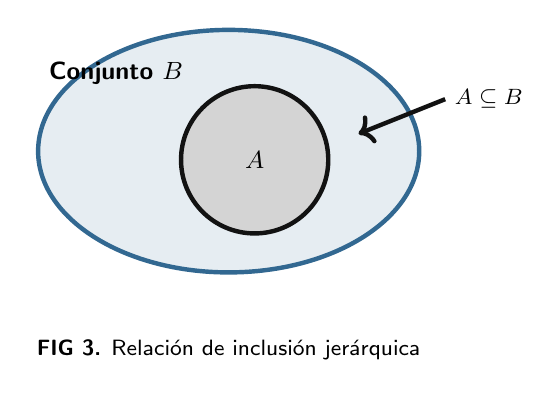
\begin{tikzpicture}[scale=1.1]
    \fill[accentblue!12] (0,0) ellipse (2.2cm and 1.4cm);
    \draw[accentblue, ultra thick] (0,0) ellipse (2.2cm and 1.4cm);
    \fill[nytblack!18] (0.3,-0.1) circle (0.85cm);
    \draw[nytblack, ultra thick] (0.3,-0.1) circle (0.85cm);
    
    \node at (-1.3, 0.9) {\small\sffamily\textbf{Conjunto $B$}};
    \node at (0.3, -0.1) {\small\sffamily\textbf{$A$}};
    
    \draw[->, nytblack, ultra thick] (2.5,0.6) -- (1.5,0.2);
    \node[right] at (2.5,0.6) {\footnotesize\sffamily $A \subseteq B$};
    
    \node at (0, -2.3) {\footnotesize\sffamily\textbf{FIG 3.} Relación de inclusión jerárquica};
\end{tikzpicture}
\end{center}

\section{Identidad y el Conjunto Vacío}

Dos conjuntos $A$ y $B$ son \textbf{iguales} ($A=B$) si y solo si contienen exactamente los mismos elementos. El \textbf{conjunto vacío} ($\emptyset$) carece de elementos pero es, paradójicamente, el concepto más fundamental: permite definir sistemas sin soluciones y garantiza que la estructura lógica nunca colapse. Es subconjunto de todo conjunto.

% --- SECCIÓN 2: NÚMEROS REALES ---
\section{Los Números Reales: Base del Análisis}

\lettrine[lines=2]{E}{l} conjunto $\mathbb{R}$ de números reales constituye la columna vertebral del análisis matemático aplicado, representando la completitud numérica absoluta necesaria para modelar fenómenos continuos.

\subsection{Estructura Tripartita}

Los números reales incluyen tres categorías exhaustivas:

\begin{enumerate}
\item \textbf{Decimales finitos:} Incluyen todos los enteros y fracciones que terminan ($\frac{3}{4} = 0.75$).
\item \textbf{Decimales infinitos periódicos:} Números racionales cuya expansión decimal se repite ($\frac{1}{3} = 0.\overline{3}$).
\item \textbf{Decimales infinitos no periódicos:} Números irracionales como $\sqrt{2}$, $\pi$, $e$.
\end{enumerate}

\begin{briefbox}{CORRESPONDENCIA BIUNÍVOCA}
Existe una relación uno a uno perfecta entre $\mathbb{R}$ y los puntos de la recta numérica dirigida (Zahlengerade), estableciendo una \textbf{geometrización completa} de la aritmética donde cada número tiene una posición única y cada posición representa un único número.
\end{briefbox}

\begin{center}
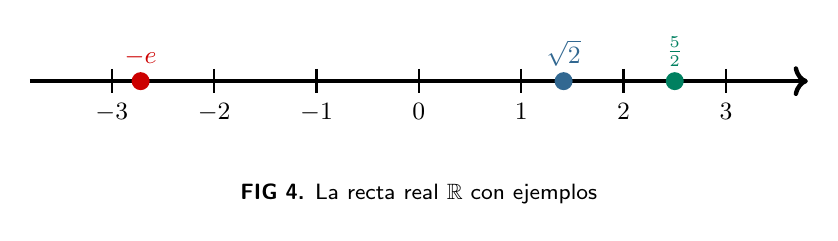
\begin{tikzpicture}[scale=1.3]
    \draw[->, ultra thick] (-3.8,0) -- (3.8,0);
    \foreach \x in {-3,-2,-1,0,1,2,3}
        \draw[thick] (\x,0.12) -- (\x,-0.12) node[below] {\small $\x$};
    
    \fill[accentblue] (1.414,0) circle (2.5pt);
    \node[above] at (1.414,0.05) {\small\color{accentblue} $\sqrt{2}$};
    
    \fill[accentred] (-2.718,0) circle (2.5pt);
    \node[above] at (-2.718,0.05) {\small\color{accentred} $-e$};
    
    \fill[accentgreen] (2.5,0) circle (2.5pt);
    \node[above] at (2.5,0.05) {\small\color{accentgreen} $\frac{5}{2}$};
    
    \node at (0, -1.1) {\footnotesize\sffamily\textbf{FIG 4.} La recta real $\mathbb{R}$ con ejemplos};
\end{tikzpicture}
\end{center}

\subsection{Operaciones y Clausura}

En $\mathbb{R}$ se definen cuatro operaciones fundamentales: adición, sustracción, multiplicación y división. Una característica esencial es la \textbf{clausura}: la suma, diferencia y producto de dos reales siempre produce otro real. Para el cociente existe la restricción absoluta de que \textbf{la división por cero no está definida}.

\subsection{Leyes Algebraicas Fundamentales}

El sistema $(\mathbb{R}, +, \cdot)$ está gobernado por tres familias de leyes:

\begin{theorembox}{LEYES CONMUTATIVAS}
\[ a + b = b + a \quad ; \quad a \cdot b = b \cdot a \]
El orden de los operandos no altera el resultado.
\end{theorembox}

\begin{theorembox}{LEYES ASOCIATIVAS}
\[ a + (b + c) = (a + b) + c \]
\[ a \cdot (b \cdot c) = (a \cdot b) \cdot c \]
La agrupación mediante paréntesis no modifica el valor final.
\end{theorembox}

\begin{theorembox}{LEY DISTRIBUTIVA}
\[ a \cdot (b + c) = a \cdot b + a \cdot c \]
Conecta multiplicación con adición, fundamento del álgebra de polinomios.
\end{theorembox}

Estas leyes no son meras conveniencias: son axiomas fundamentales que garantizan la consistencia de todas las operaciones algebraicas superiores, incluyendo el álgebra de vectores y matrices.

\section{Orden, Inecuaciones y Valor Absoluto}

\subsection{Anordnung der Zahlen}

Para cualquier par de números reales $a, b \in \mathbb{R}$, se cumple exactamente una de tres relaciones mutuamente excluyentes: $a < b$, $a = b$, o $a > b$. Esta \textbf{tricotomía} es la esencia del orden total en $\mathbb{R}$.

\textbf{Interpretación Geométrica:}
\begin{itemize}
\item $a < b$: El punto $a$ se sitúa a la \textbf{izquierda} de $b$ en la recta
\item $a > b$: El punto $a$ se sitúa a la \textbf{derecha} de $b$
\item $a = b$: Ambos puntos coinciden espacialmente
\end{itemize}

\subsection{Transformaciones de Inecuaciones}

Las inecuaciones se resuelven mediante \textbf{transformaciones equivalentes} que preservan el conjunto solución:

\begin{examplebox}{REGLAS FUNDAMENTALES}
\textbf{1. Adición/Sustracción:} Sumar o restar cualquier término $T(x)$ en ambos lados preserva el signo de desigualdad.

\textbf{2. Multiplicación por positivos:} Si $c > 0$:
$$a < b \Rightarrow ac < bc$$

\textbf{3. Multiplicación por negativos:} Si $c < 0$, el signo se invierte:
$$a < b \Rightarrow ac > bc$$
\end{examplebox}

\begin{warningbox}{ADVERTENCIA CRÍTICA}
Cuando se multiplica o divide por un término variable $T(x)$, se debe realizar \textbf{distinción de casos} (Fallunterscheidung) según el signo de $T(x)$ en diferentes intervalos.
\end{warningbox}

\begin{examplebox}{INECUACIÓN RACIONAL CON DISTINCIÓN DE CASOS}
Resolver: $\frac{2x-1}{x+2} > 3$

\textbf{Caso 1:} $x+2 > 0$ (es decir, $x > -2$)
$$2x-1 > 3(x+2) \Rightarrow x < -7$$
Contradicción con $x > -2$: sin soluciones válidas.

\textbf{Caso 2:} $x+2 < 0$ (es decir, $x < -2$)
$$2x-1 < 3(x+2) \Rightarrow x > -7$$
Intersección: $-7 < x < -2$ ✓

\textbf{Solución final:} $L = \{x \mid -7 < x < -2\} = (-7,-2)$
\end{examplebox}

\subsection{Valor Absoluto: Función de Distancia}

El \textbf{valor absoluto} $|a|$ representa la distancia del número $a$ al origen en la recta numérica.

\begin{theorembox}{DEFINICIÓN POR CASOS}
\[ |a| = \begin{cases} 
a & \text{si } a \geq 0 \\
-a & \text{si } a < 0
\end{cases} \]
\end{theorembox}

\textbf{Propiedades Fundamentales:}
\begin{itemize}
\item $|a| \geq 0$ para todo $a \in \mathbb{R}$
\item $|x - a|$ mide la distancia entre $x$ y $a$
\item $|a \cdot b| = |a| \cdot |b|$
\item Desigualdad triangular: $|a + b| \leq |a| + |b|$
\end{itemize}

\begin{center}
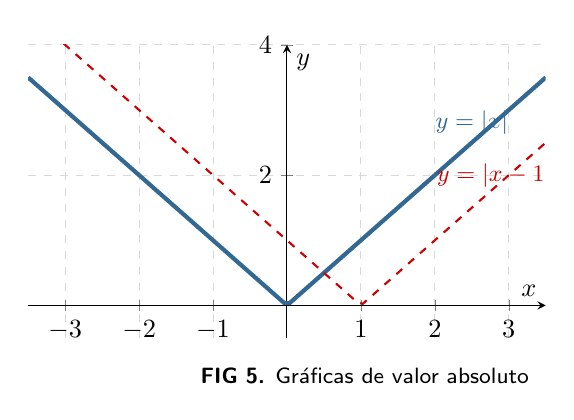
\begin{tikzpicture}[scale=0.95]
    \begin{axis}[
        axis lines=middle,
        xlabel={$x$},
        ylabel={$y$},
        domain=-3.5:3.5,
        samples=100,
        width=8.5cm,
        height=5.5cm,
        ymin=-0.5, ymax=4,
        grid=major,
        grid style={dashed, gray!30}
    ]
    \addplot[accentblue, ultra thick] {abs(x)};
    \addplot[accentred, dashed, thick] {abs(x-1)};
    \node at (axis cs: 2.5,2.8) {\small\color{accentblue} $y = |x|$};
    \node at (axis cs: 2.8,2) {\small\color{accentred} $y = |x-1|$};
    \end{axis}
    \node at (4.5, -0.5) {\footnotesize\sffamily\textbf{FIG 5.} Gráficas de valor absoluto};
\end{tikzpicture}
\end{center}

\subsection{Ecuaciones con Valor Absoluto}

Las ecuaciones que contienen términos con valor absoluto requieren \textbf{distinción de casos} basada en el signo del argumento.

\begin{examplebox}{RESOLUCIÓN EXHAUSTIVA POR CASOS}
Resolver: $|x + 2| - 2|x - 3| = 4$

\textbf{Puntos críticos:} $x = -2$ y $x = 3$ dividen la recta en tres intervalos.

\textbf{Caso I} ($x < -2$): Ambos argumentos negativos
$$-(x+2) - 2[-(x-3)] = 4$$
$$-x-2+2x-6 = 4 \Rightarrow x = 12$$
$12 \not< -2$: solución falsa (Scheinlösung) ✗

\textbf{Caso II} ($-2 \leq x \leq 3$): Primer argumento positivo, segundo negativo
$$(x+2) - 2[-(x-3)] = 4$$
$$x+2+2x-6 = 4 \Rightarrow 3x = 8 \Rightarrow x = \frac{8}{3}$$
$\frac{8}{3} \approx 2.67 \in [-2,3]$: solución válida ✓

\textbf{Caso III} ($x > 3$): Ambos argumentos positivos
$$(x+2) - 2(x-3) = 4$$
$$x+2-2x+6 = 4 \Rightarrow x = 4$$
$4 > 3$: solución válida ✓

\textbf{Conjunto solución:} $L = \left\{\frac{8}{3}, 4\right\}$
\end{examplebox}

\begin{warningbox}{VERIFICACIÓN OBLIGATORIA}
Siempre se debe verificar cada solución candidata en la ecuación original para descartar soluciones falsas generadas por transformaciones no equivalentes.
\end{warningbox}

% --- SECCIÓN 3: ECUACIONES ---
\section{Teoría Exhaustiva de Ecuaciones}

\subsection{Ecuaciones Lineales}

La forma canónica $ax + b = 0$ con $a \neq 0$ posee exactamente una solución:
\[ x = -\frac{b}{a} \]

Esta solución única refleja la estructura de campo de $\mathbb{R}$.

\subsection{Ecuaciones Cuadráticas}

La forma general $ax^2 + bx + c = 0$ se normaliza dividiendo por $a$ para obtener $x^2 + px + q = 0$ donde $p = b/a$ y $q = c/a$.

\begin{theorembox}{FÓRMULA $p,q$ (FORMA NORMALIZADA)}
\[ x_{1,2} = -\frac{p}{2} \pm \sqrt{\left(\frac{p}{2}\right)^2 - q} \]
\end{theorembox}

El \textbf{discriminante} $D = \left(\frac{p}{2}\right)^2 - q$ determina completamente la naturaleza de las soluciones:

\begin{center}
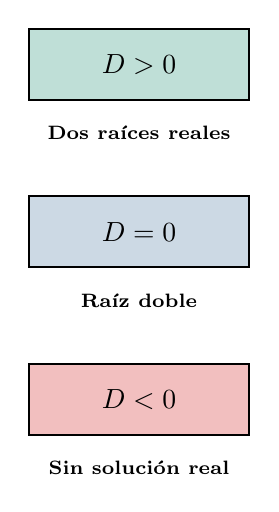
\begin{tikzpicture}[node distance=1.5cm]
    \node[draw, fill=accentgreen!25, rectangle, minimum width=2.8cm, minimum height=0.9cm, thick] (pos) {$D > 0$};
    \node[below=0.2cm of pos] {\scriptsize\textbf{Dos raíces reales}};
    
    \node[draw, fill=accentblue!25, rectangle, minimum width=2.8cm, minimum height=0.9cm, thick, below=1.2cm of pos] (zero) {$D = 0$};
    \node[below=0.2cm of zero] {\scriptsize\textbf{Raíz doble}};
    
    \node[draw, fill=accentred!25, rectangle, minimum width=2.8cm, minimum height=0.9cm, thick, below=1.2cm of zero] (neg) {$D < 0$};
    \node[below=0.2cm of neg] {\scriptsize\textbf{Sin solución real}};
\end{tikzpicture}
\end{center}

\subsection{Ecuaciones de Grado Superior}

\begin{theorembox}{TEOREMA FUNDAMENTAL DEL ÁLGEBRA}
Una ecuación polinómica de grado $n$ tiene como máximo $n$ soluciones reales.
\end{theorembox}

\subsubsection{Ecuaciones Bicuadráticas}

Para $ax^4 + bx^2 + c = 0$:

\begin{examplebox}{MÉTODO DE SUBSTITUCIÓN}
\textbf{Paso 1:} Sustituir $u = x^2$: $au^2 + bu + c = 0$

\textbf{Paso 2:} Resolver en $u$ con fórmula cuadrática.

\textbf{Paso 3:} Para cada $u_i > 0$: $x = \pm\sqrt{u_i}$
\end{examplebox}

\subsubsection{Esquema de Horner}

Método eficiente para división sintética. Si $x_1$ es raíz de $P(x)$, permite dividir por $(x-x_1)$ y reducir el grado.

\subsection{Ecuaciones Irracionales}

Contienen la incógnita bajo radicales.

\begin{warningbox}{ADVERTENCIA CRÍTICA}
Elevar al cuadrado NO es transformación equivalente. Pueden aparecer \textbf{soluciones falsas}. La verificación es \textbf{OBLIGATORIA}.
\end{warningbox}

\section{Sistemas de Ecuaciones Lineales}

Un sistema de $m$ ecuaciones con $n$ incógnitas se representa:
\[ A\mathbf{x} = \mathbf{c} \]

\subsection{Representación Matricial}

\begin{theorembox}{COMPONENTES DEL SISTEMA}
\textbf{Matriz de coeficientes:}
$A = \begin{pmatrix} a_{11} & \cdots & a_{1n} \\ \vdots & \ddots & \vdots \\ a_{m1} & \cdots & a_{mn} \end{pmatrix}$

\textbf{Vector solución:}
$\mathbf{x} = \begin{pmatrix} x_1 \\ \vdots \\ x_n \end{pmatrix}$

\textbf{Vector constante:}
$\mathbf{c} = \begin{pmatrix} c_1 \\ \vdots \\ c_m \end{pmatrix}$
\end{theorembox}

\subsection{Algoritmo de Gauss}

Transforma el sistema en forma escalonada mediante:

\begin{enumerate}
\item Intercambiar ecuaciones
\item Multiplicar ecuación por constante no nula
\item Sumar múltiplo de una ecuación a otra
\end{enumerate}

\subsection{Análisis de Solubilidad}

\begin{theorembox}{CRITERIO FUNDAMENTAL}
Sistema resoluble $\Leftrightarrow$ $Rg(A) = Rg(A|\mathbf{c})$
\end{theorembox}

\textbf{Casos según rango $r$:}
\begin{itemize}
\item $r = n$: Solución única
\item $r < n$: Infinitas soluciones ($n-r$ parámetros libres)
\item $Rg(A) < Rg(A|\mathbf{c})$: Sin solución
\end{itemize}

\subsection{Regla de Cramer}

Para sistemas cuadrados con $\det(A) \neq 0$:
\[ x_i = \frac{\det(A_i)}{\det(A)} \]

\subsection{Aplicación: Circuitos Eléctricos}

\begin{examplebox}{ANÁLISIS DE RED CON KIRCHHOFF}
Para circuito con resistencias $R_1, R_2, R_3$ y tensión $U$:

\textbf{Regla de nudos:}
$I_1 - I_2 - I_3 = 0$

\textbf{Reglas de mallas:}
$R_1 I_1 + R_2 I_2 = U$
$R_2 I_2 - R_3 I_3 = 0$

\textbf{Matriz del sistema:}
$A = \begin{pmatrix} 1 & -1 & -1 \\ R_1 & R_2 & 0 \\ 0 & R_2 & -R_3 \end{pmatrix}$
\end{examplebox}

\begin{center}
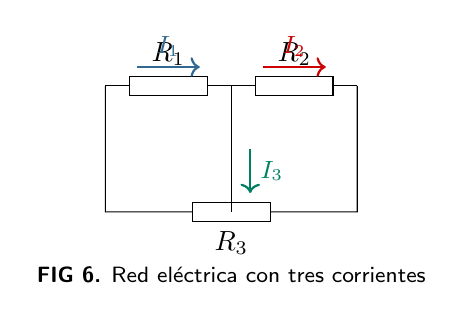
\begin{tikzpicture}[scale=0.8, circuit ee IEC]
    \draw (0,0) to [resistor={info={$R_1$}}] (2,0)
          to [resistor={info={$R_2$}}] (4,0);
    \draw (4,0) -- (4,-2) to [resistor={info={$R_3$}}] (0,-2) -- (0,0);
    \draw (2,0) -- (2,-2);
    \draw[->, thick, accentblue] (0.5,0.3) -- (1.5,0.3) node[midway, above] {\small $I_1$};
    \draw[->, thick, accentred] (2.5,0.3) -- (3.5,0.3) node[midway, above] {\small $I_2$};
    \draw[->, thick, accentgreen] (2.3,-1) -- (2.3,-1.7) node[midway, right] {\small $I_3$};
    \node at (2, -3) {\footnotesize\sffamily\textbf{FIG 6.} Red eléctrica con tres corrientes};
\end{tikzpicture}
\end{center}

\section{Triángulo de Pascal}

Esquema numérico para coeficientes binomiales $\binom{n}{k}$.

\begin{theorembox}{CONSTRUCCIÓN RECURSIVA}
\textbf{Bordes:} Todos son 1

\textbf{Interior:} Cada número es la suma de los dos superiores:
$\binom{n}{k} + \binom{n}{k+1} = \binom{n+1}{k+1}$
\end{theorembox}

\begin{center}
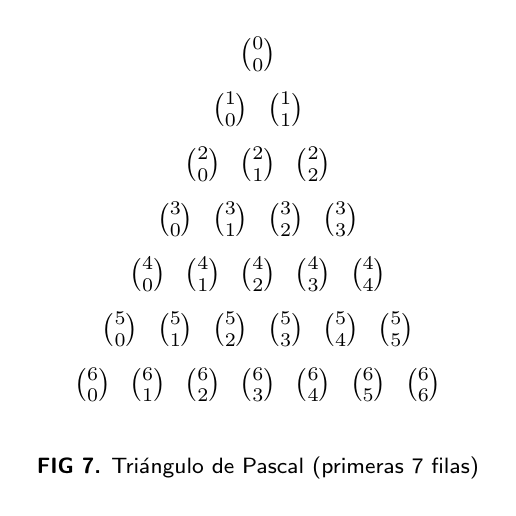
\begin{tikzpicture}[scale=0.7]
\foreach \n in {0,...,6} {
  \foreach \k in {0,...,\n} {
    \node at (\k-\n/2, -\n) {$\binom{\n}{\k}$};
  }
}
\node at (0, -7.5) {\footnotesize\sffamily\textbf{FIG 7.} Triángulo de Pascal (primeras 7 filas)};
\end{tikzpicture}
\end{center}

\textbf{Aplicación:} Desarrollo del binomio de Newton:
$(a+b)^n = \sum_{k=0}^{n} \binom{n}{k} a^{n-k} b^k$

\section{Método de Newton}

Para ecuaciones sin solución analítica, el método iterativo de Newton proporciona aproximaciones:

\begin{theorembox}{FÓRMULA ITERATIVA}
\[ x_{n+1} = x_n - \frac{f(x_n)}{f'(x_n)} \]
\end{theorembox}

Convergencia cuadrática cerca de la raíz.

\begin{center}
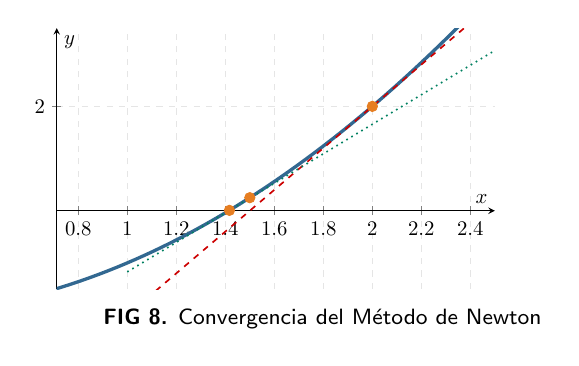
\begin{tikzpicture}[scale=0.75]
    \begin{axis}[
        axis lines=middle,
        xlabel={$x$},
        ylabel={$y$},
        domain=0.5:4,
        samples=100,
        width=9cm,
        height=6cm,
        ymin=-1.5, ymax=3.5,
        grid=major,
        grid style={dashed, gray!20}
    ]
    \addplot[accentblue, ultra thick] {x^2 - 2};
    \addplot[accentred, dashed, thick, domain=1:3] {4*x - 6};
    \addplot[accentgreen, dotted, thick, domain=1:2.5] {2.8284*x - 4};
    
    \addplot[mark=*, only marks, mark size=2.5pt, accentorange] coordinates {(2,2) (1.5,0.25) (1.4167,0.007)};
    
    \node at (axis cs: 3.2,2) {\small\color{accentblue} $f(x)$};
    \end{axis}
    \node at (4.5, -0.5) {\footnotesize\sffamily\textbf{FIG 8.} Convergencia del Método de Newton};
\end{tikzpicture}
\end{center}

\section{Conclusión Técnica}

Los fundamentos matemáticos constituyen el andamiaje sobre el cual se erigen las disciplinas científico-técnicas. La teoría de conjuntos proporciona el lenguaje, los números reales la métrica, las ecuaciones el mecanismo de modelado, y los sistemas lineales la estructura para problemas multivariables.

En el rigor de la ingeniería moderna, según Papula, solo la precisión lógica y coherencia estructural garantizan resultados confiables.

\vspace{0.5cm}
\begin{briefbox}{REFERENCIAS BIBLIOGRÁFICAS}
\textbf{Fuente Principal:} Papula, L. (2024). \textit{Mathematik für Ingenieure und Naturwissenschaftler, Band 1} (16.ª ed.). Springer Vieweg. ISBN 978-3-658-45801-0. DOI: 10.1007/978-3-658-45802-7

\textbf{Investigador:} Emanuel Quintana Silva, Economista en formación (Universidad Pedagógica y Tecnológica de Colombia). Especialización en Econometría Computacional y aplicaciones de R/Python. 

\textbf{Contacto:} emanuel.quintana@uptc.edu.co | ORCID: 0009-0006-8419-2805
\end{briefbox}

\vspace{1cm}
\begin{center}
    \color{nytgray}
    \rule{0.45\linewidth}{0.8pt} \\
    \vspace{0.15cm}
    \small\sffamily PRÓXIMA EDICIÓN: ÁLGEBRA VECTORIAL Y GEOMETRÍA ANALÍTICA
    \vspace{0.1cm}
    
    \rule{0.45\linewidth}{0.8pt}
    
    \vspace{0.3cm}
    \footnotesize THE SCIENCE TIMES | ENERO 2026
\end{center}

\end{document}